\newpage

\section*{Task 2}

Starting with the following function expressed in maxterms:
\[
    f(d,c,b,a)=\prod{(M_{0},M_{1},M_{5},M_{7},M_{8},M_{10},M_{14},M_{15})}
\]

Taking $d,c,b,a$ as input variables. For simplify, the same 
function is expressed in minterms to operate later:
\[
    f(d,c,b,a)=\sum{(m_{2},m_{3},m_{4},m_{6},m_{9},m_{11},m_{12},m_{13})}
\]

Starting with it, we build the function without simplifying:
\[
    f(d,c,b,a)=(\overline{d} \cdot \overline{c} \cdot b \cdot \overline{a})+
    (\overline{d} \cdot \overline{c} \cdot b \cdot a)+
    (\overline{d} \cdot c \cdot \overline{b} \cdot \overline{a})+
    (\overline{d} \cdot c \cdot b \cdot \overline{a})+
    (d \cdot \overline{c} \cdot \overline{b} \cdot a)+
    (d \cdot \overline{c} \cdot b \cdot a)+
    (d \cdot c \cdot \overline{b} \cdot \overline{a})+
    (d \cdot c \cdot \overline{b} \cdot a)
\]

We grouped by common factor in a convenient way:
\begin{eqnarray}
    \nonumber f(d,c,b,a)&=&\underbrace{(\overline{d} \cdot \overline{c} \cdot b \cdot \overline{a})+
    (\overline{d} \cdot \overline{c} \cdot b \cdot a)}+\underbrace{
    (\overline{d} \cdot c \cdot \overline{b} \cdot \overline{a})+
    (\overline{d} \cdot c \cdot b \cdot \overline{a})}+\underbrace{
    (d \cdot \overline{c} \cdot \overline{b} \cdot a)+
    (d \cdot \overline{c} \cdot b \cdot a)}+\\
    \nonumber &\longrightarrow&\underbrace{(d \cdot c \cdot \overline{b} \cdot \overline{a})+
    (d \cdot c \cdot \overline{b} \cdot a)}
\end{eqnarray}
\[
    f(d,c,b,a)=[\overline{d} \cdot \overline{c} \cdot b \cdot \underbrace{(\overline{a}+a)}_1]+
    [\overline{d} \cdot c \cdot \overline{a} \cdot \underbrace{\overline{b}+b)}_1]+
    [d \cdot \overline{c} \cdot a \cdot  \underbrace{(\overline{b}+b)}_1]+
    [d \cdot c \cdot \overline{b} \cdot \underbrace{(\overline{a}+a)}_1]
\]
\[
    \boxed{f(d,c,b,a)=(\overline{d} \cdot \overline{c} \cdot b)+
    (\overline{d} \cdot c \cdot \overline{a})+
    (d \cdot c \cdot \overline{b})+
    (d \cdot \overline{c} \cdot a)}
\]
\\ %Salto de linea
Analogously, starting with the expresssion in minterms we reduce 
the function through a map of Karnaugh:

\begin{centering}
    \begin{Karnaugh}
        \minterms{2,3,4,6,9,11,12,13}
        \maxterms{0,1,5,7,8,10,14,15}
        \implicant{3}{2}{red}
        \implicantcostats{4}{6}{red}
        \implicant{12}{13}{red}
        \implicant{9}{11}{red}
    \end{Karnaugh}
\par\end{centering}

From the first group (first row) we have that $d$, $c$ and $b$ 
are constantes, thus the first factor stays the way 
$ \overline{d} \overline{c} b$.\par
From the second group (second row) we have $d$, $c$ and $a$ as
constants, thus this factor stays as $ \overline{d} c \overline{a}$.\par
From the third group (third row) remain constant $d$, $c$ and $b$, thus 
this factor stays as $d c \overline{b}$.\par
Finally, from the last row, in the group $d$, $c$ and $a$ stay constant, 
thus this factor stays the way
$d \overline{c} a$.\par
Adding the partial termns we get the simplified function:
\[
    \boxed{f(d,c,b,a)=(\overline{d} \cdot \overline{c} \cdot b)+
    (\overline{d} \cdot c \cdot \overline{a})+
    (d \cdot c \cdot \overline{b})+
    (d \cdot \overline{c} \cdot a)}
\]
Wich is the same obtained by simplification by boolean algebra. \par
Taking this function, it was implemented in a logical circuit
 by AND, OR and NOT gates, as shown below.

\begin{figure}[H]
    \begin{centering}
    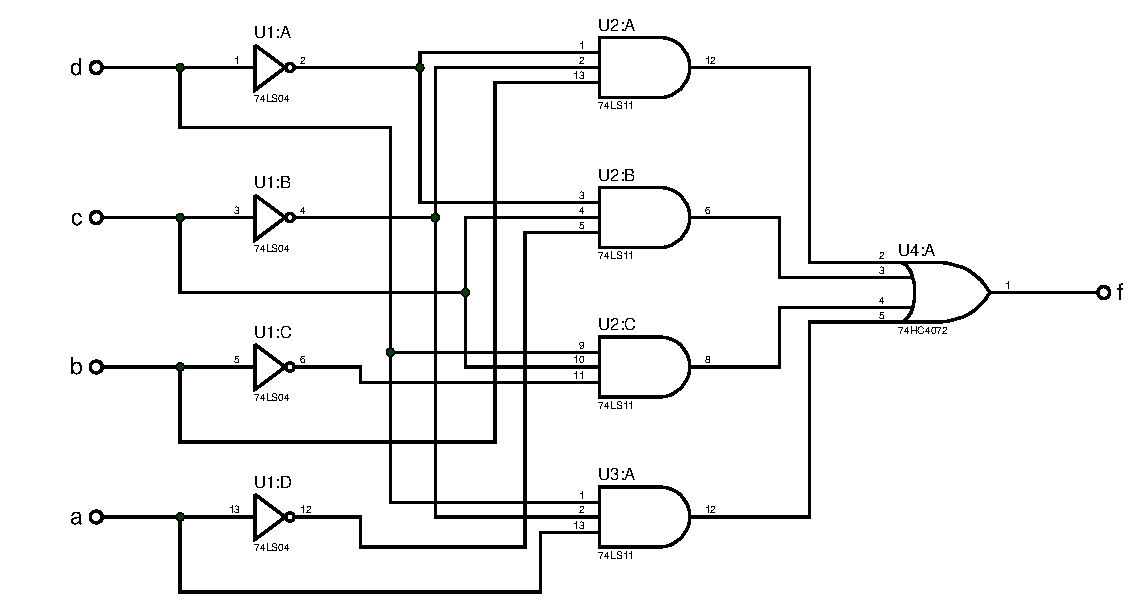
\includegraphics[width=1\textwidth]{data/ImplementacionEj2}
    \par\end{centering}
    \caption{Logical circuit that implements $f(d,c,b,a)$ - Made in Proteus 7.8}
\end{figure}

For implementation using only NOR gates, first we have to work
 with the obtained function applyin boolean algebra properties. 
 Taking the function:
\[
    f(d,c,b,a)=(\overline{d} \cdot \overline{c} \cdot b)+
    (\overline{d} \cdot c \cdot \overline{a})+
    (d \cdot c \cdot \overline{b})+
    (d \cdot \overline{c} \cdot a)
\]
\par
We twice denied the terms separated by sums, for keeping the equal:
\[
    f(d,c,b,a)=\overline{\overline{(\overline{d} \cdot \overline{c} \cdot b)}}+
    \overline{\overline{(\overline{d} \cdot c \cdot \overline{a})}}+
    \overline{\overline{(d \cdot c \cdot \overline{b})}}+
    \overline{\overline{(d \cdot \overline{c} \cdot a)  }}
\]
\par
Next we deny the factors only once, for turning the products 
into sums (property of De Moivre):
\[
    \boxed{f(d,c,b,a)=\overline{(d+c+\overline{b})}+
    \overline{(d+\overline{c}+a)}+
    \overline{(\overline{d}+\overline{c}+b)}+
    \overline{(\overline{d}+c+\overline{a})}}
\]
\par

Having the expression in terms of sums, it is possible to implement 
the circuit using only NOR gates, as shown below.

\begin{figure}[H]
    \begin{centering}
    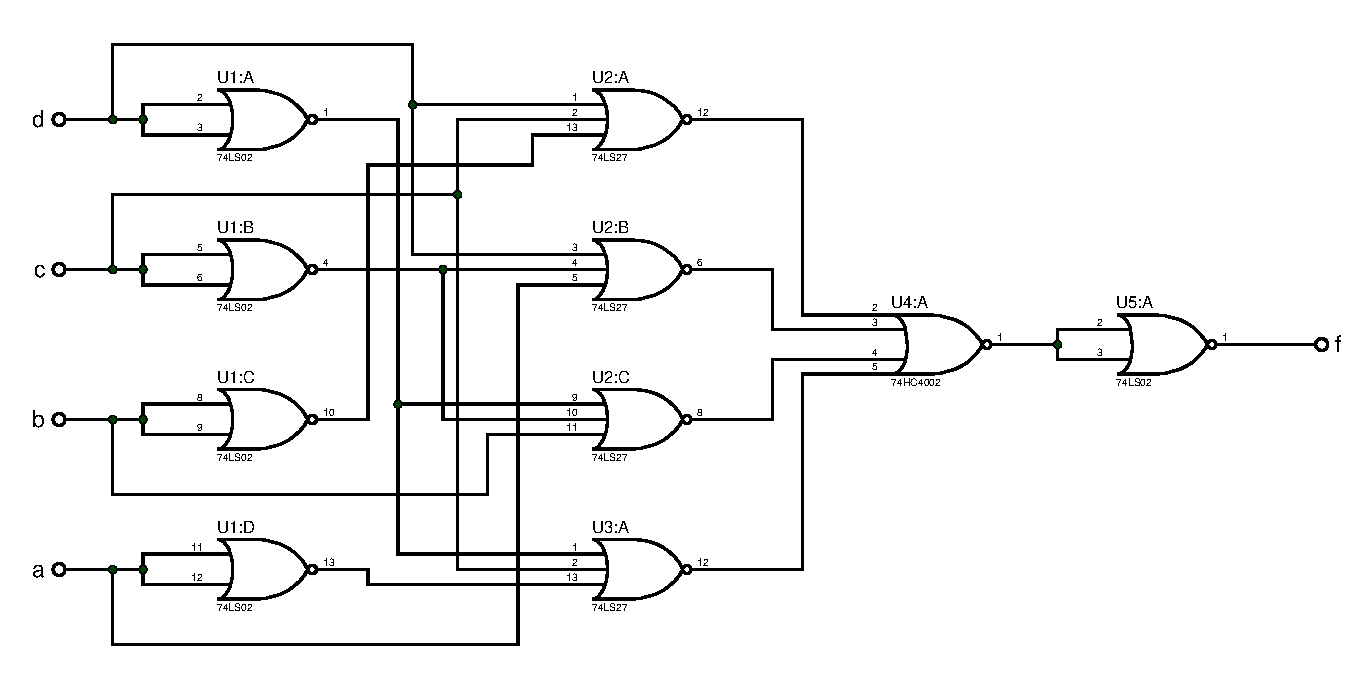
\includegraphics[width=1\textwidth]{data/ImplementacionEj2_NOR}
    \par\end{centering}
    \caption{Logical circuit that implements $f(d,c,b,a)$
    with NOR gates - Made in Proteus 7.8}
\end{figure}


